\section{View und Controller}
\subsection{View}\label{subsec:View}
Der View dient der Darstellung der Tableau-Anwendung für den Anwender. Er besteht im Kern aus einem HTML-Dokument (Unterabschnitt \ref{subsubsec:HTML}) und einer clientseitigen Logik, die den DOM-Tree des HTML-Dokuments manipuliert. Die clientseitige Logik hat zwei Bestandteile, also \textit{TableauClient.js} (Unterabschnitt \ref{subsubsec:TableauClient} ) und Klasse \textit{TableauView} (Unterabschnitt \ref{subsubsec:TableauView}).
\subsubsection{HTML-Dokument} \label{subsubsec:HTML}
Das folgendes HTML-Dokument (Listing \ref{lis:HTMLhead} und \ref{lis:HTMLbody}) wird genutzt, um die Anwendung einzublenden. Abbildung  \ref{figs:screenshot-GUI} zeigt dabei einen Screenshot der Anwendung in der Desktop- und Mobile-Version.

\lstinputlisting[language=HTML, caption=HTML-head, basicstyle=\scriptsize, label={lis:HTMLhead}]{head.html}

Diese \textit{head}-Tags enthalten den Titel für benötige Dokumente, Skripte und Metainformationen. In den \textit{link}-Tags wird Bootstrap-Framework und das benutzerdefinierte Stylesheet \textit{style.css} verknüpft. In den \textit{script}-Tags werden die clientseitigen Skripts definiert. Hierbei wird \textit{require.js} verwendet um JS-Dateien zu importieren. \textit{jquery.min.js} und \textit{bootstrap.min.js} werden verwendet um jQuery-Bibliothek und Bootstrap-JavaScript-Plugins einzubinden und \textit{loader.js} wird verwendet um Google-Chart Loader zu laden.

\lstinputlisting[basicstyle=\scriptsize, style=myCustomHTMLStyle, caption=HLML-body, label={lis:HTMLbody}]{body.html}

Wie in Unterabschnitt \ref{Bootstrap} erwähnt, ist die Benutzeroberfläche der Tableau-
Anwendung als eine Responsive-Website mit ``Laptop-First'' Strategie (Bildschirmgröße $\geq$ 768 px) implementiert. Daher wird das Layout der Seite basierend auf der Klasse \textit{.col-md-} von der Bootstrap Grid-System angeordnet und angepasst.

\begin{figure}[ !h] \centering
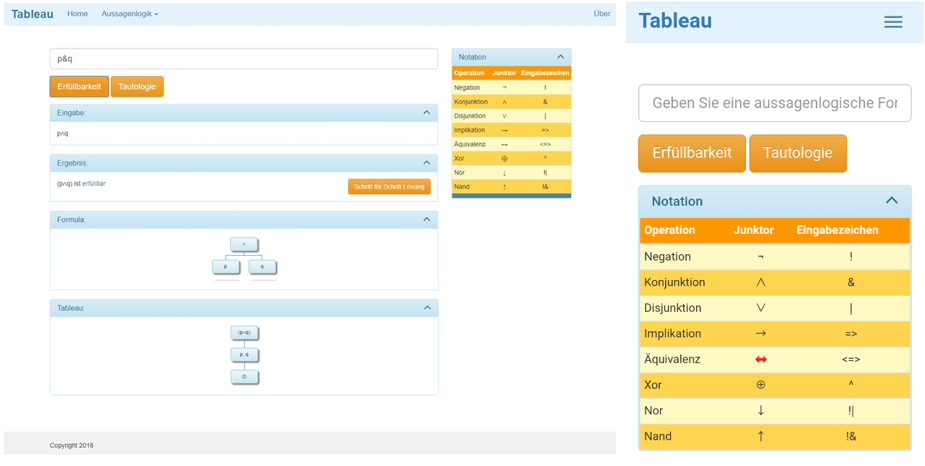
\includegraphics[width=1.0\textwidth]{screenshot-GUI}
\caption[Screenshots der Tableau-Anwendung]{Screenshots der Tableau-Anwendung für Desktop-(links) und Mobile-Version(rechts)}\label{figs:screenshot-GUI}
\end{figure}

\subsubsection{\textit{TableauClient.js} als Schnittstelle zum HTML-Dokument} \label{subsubsec:TableauClient}
Der View wird im Browser initial durch obiges HTML-Dokument erzeugt. Im Verlaufe der Anwendung wird der DOM-Tree dieses HTML-Dokuments durch die Klasse \textit{TableauView} manipuliert, um den Anwendungszustand darzustellen. Die Klasse \textit{TableauView} wird dabei durch das Skript \textit{TableauClient.js}, das die Nutzerinteraktionen ermöglicht, geladen. In dem  Skript \textit{TableauClient.js} werden die folgenden Funktionen implementiert. Hier gibt es eine Beachtung, dass diese Funktionen wie normale JavaScript-Funktionen implementiert werden und nicht vom einem Objekt-Namespace z.B \textit{MyObj.theMethod()} aufgerufen werden.

\begin{itemize}
\item	\textit{pressTautologyButton()}: Diese Funktion wird ausgeführt, wenn der Anwender auf den Button  ``Tautologie'' drückt. Sie initialisiert  eine Instanz der Klasse \textit{TableauView} und ruft die Methode \textit{checkTautology()} der Instanz auf.
\item \textit{pressSatisfiableButton()}: Diese Funktion wird ausgeführt, wenn der Anwender auf den Button  ``Erfüllbarkeit'' drückt. Sie initialisiert eine Instanz der Klasse \textit{TableauView} und ruft die Methode \textit{checkSatisfiable()} der Instanz auf.
\item	\textit{stepByStepSolution()}: Diese Funktion wird ausgeführt, wenn der Anwender auf den Button  ``Schritt für Schritt Lösung'' drückt. Über dem Aufruf der Methode \textit{stepByStepSolutionOutput()} von der Klasse \textit{TableauView} leitet sie diese  Benutzerinteraktion an eine Instanz der Klasse \textit{TableauView} weiter.
\item	\textit{pressNextStepButton()}: Diese Funktion wird ausgeführt, wenn der Anwender auf den Button  ``Nächste Schritt''  mit der Id \textit{nextStepButton} des DOM-Trees  drückt. Über dem Aufruf der Methode \textit{nextSolutionStepOutput()} von der Klasse \textit{TableauView} leitet sie diese Benutzerinteraktion an eine Instanz der Klasse \textit{TableauView} weiter.
\end{itemize}

Außerdem enthält \textit{TableauClient.js} die folgenden Funktionen. Die Funktionen werden von Google Charts unterstützt um die  Organigramme auf der Webseite zeichnet zu lassen. 
\begin{itemize}
\item	\textit{drawFormulaChart()}: Visualisiert die Darstellung der Formel mittels Google Charts. Diese Darstellung wird in das DIV-Element mit der Id \textit{Formula\_chart\_div} des DOM-Trees eingeblendet.
\item	\textit{drawTableauChart()}: Visualisiert die Darstellung des Tableau ohne Regel-Bezeichnungen mittels Google Charts. Diese Darstellung wird in das DIV-Element mit der Id \textit{Tableau\_chart\_div} des DOM-Trees eingeblendet.
\item	\textit{drawTableauChartStepByStep()}: Visualisiert teilweise die Darstellung des Tableau mittels Google Charts.
\item	\textit{drawTableauChartWithRule()}: Visualisiert die Darstellung des Tableau mit Regel-Bezeichnungen mittels Google Charts. Diese Darstellung wird in das DIV-Element mit der Id \textit{stepByStepDiagram} des DOM-Trees eingeblendet.
\begin{lstlisting}[language=JavaScript, caption= drawTableauChart() (TableauClient.js), basicstyle=\scriptsize] 
function drawTableauChart() {
    TableauChartData = new google.visualization.DataTable();
    var arrOfTableauNodes = view.controller.rootTableau.getTableauForChart();
    // For each orgchart box, provide the label, and the parentNode
    TableauChartData.addColumn('string', 'Label');
    TableauChartData.addColumn('string', 'Parent');
    TableauChartData.addRows(arrOfTableauNodes);
    // Create the chart.
    var chart = new google.visualization.OrgChart(document.getElementById('Tableau_chart_div'));
    // Draw the chart, setting the allowHtml option to true for the tooltips.
    chart.draw(TableauChartData, {allowHtml: true});
}
\end{lstlisting}
\end{itemize}

\subsubsection{TableauView} \label{subsubsec:TableauView}
\begin{figure}[ !h] \centering
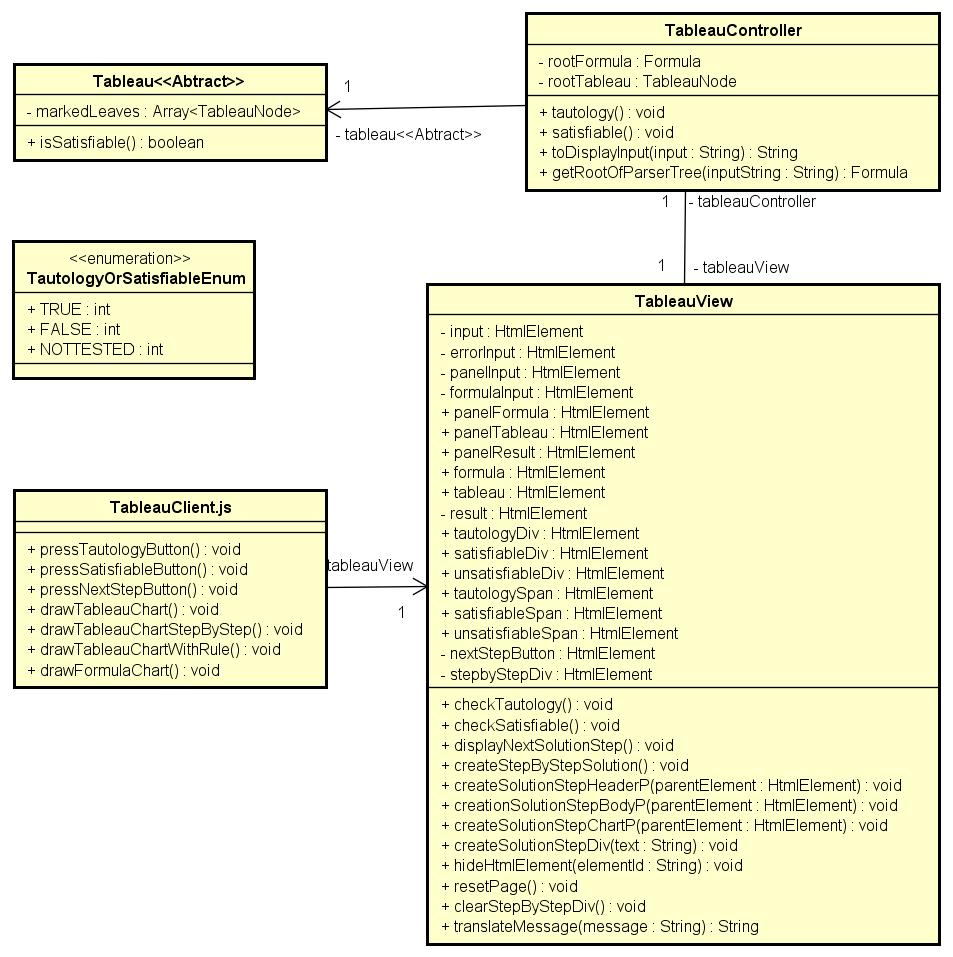
\includegraphics[width=1.0\textwidth]{ClassDiagramViewController}
\caption[KlassendiagrammControllerView]{Klassendiagramm (View und Controller)}\label{fig:KlassendiagrammControllerView}
\end{figure}
Folgende Elemente haben dabei eine besondere Bedeutung und können dabei über entsprechende Attribute der Klasse \textit{TableauView} (Abbildung \ref{fig:KlassendiagrammControllerView}) angesprochen werden.
\begin{itemize}
\item	\textit{input}: Das Element mit dem Identifier \textit{input} dient dazu die Eingabe zu erhalten.
\item	\textit{errorInput}: Das Element mit dem Identifier \textit{errorInput} dient dazu ein Warnungstext bei fehlerhaften Eingaben einzublenden.
\item	\textit{panelInput}: Das Element mit dem Identifier \textit{panel-input} wird genutzt, um die Tafel, die die Eingabeformel enthält, einzublenden.
\item	\textit{formulaInput}: Das Element mit dem Identifier \textit{ formulaInput} dient dazu die Eingabeformel einzublenden.
\item	\textit{panelFormula}, \textit{panelTableau} und\textit{ panelResul}t : Die Elemente mit dem Identifier \textit{panel-formula}, \textit{panel-tableau} und \textit{panel-result} werden genutzt, um die Tafeln, die die Darstellung der Formel, die Darstellung des Tableau und  das Prüfungsergebnis (z.B. dass die Eingabeformel erfüllbar oder Tautologie ist) enthält, einzublenden.
\item	\textit{formula}, \textit{tableau} und \textit{result} : Die Elemente mit dem Identifier \textit{formula}, \textit{tableau} und \textit{resul}t   werden genutzt, um die Panel-Bodys der Panel \textit{panel-formula}, \textit{panel-tableau} und \textit{panel-result} einzublenden.
\item	\textit{tautologyDiv},\textit{ satisfiableDiv} und \textit{unsatisfiableDiv}: Die Elemente mit dem Identifier \textit{tautologyDiv},  \textit{satisfiableDiv}, \textit{unsatisfiableDiv} dient dazu die Prüfungsergebnisse einzublenden.
\item	\textit{tautologySpan}, \textit{satisfiableSpan} und \textit{unsatisfiableSpan}:	Die Element mit dem Identifier  \textit{tautologySpan}, \textit{satisfiableSpan} und  \textit{unsatisfiableSpan} dient dazu die Prüfungsergebnistexte einzublenden.
\item	\textit{nextStepButton}: Das Element mit dem Identifier \textit{nextStepButton} wird genutzt, um das Button ``Nächste Schritt'' im Popup-Fenster ``Schritt für Schritt Lösung'' einzublenden.
\item	\textit{stepByStepDiv}: Das Element mit dem Identifier \textit{stepByStepDiv} wird genutzt, um die Lösung im Popup-Fenster ``Schritt für Schritt Lösung'' einzublenden.
\end{itemize}

\textit{TableauView} kann mittels folgender Methoden den DOM-Tree manipulieren:
\begin{itemize}
\item	\textit{checkTautology()}: Mittels der Methode \textit{toDisplayInput()} des Controllers enthält sie die formatierende Eingabeformel, die in das DIV-Element mit der Id \textit{formulaInput} des DOM-Trees eingeblendet wird. Sie ruft die Methode \textit{tautology()} des Controllers auf um das Tableau und das Ergebnis der Tautologie-Prüfung einzublenden. Bei fehlerhafter Eingaben gibt sie eine Fehlermeldung aus. Diese Fehlermeldung wird in das DIV-Element mit der Id \textit{errorInput} des DOM-Trees eingeblendet.
\begin{lstlisting}[language=JavaScript, caption= checkTautology()(Klasse TableauView), basicstyle=\scriptsize] 
TableauView.prototype.checkTautology = function () {
    this.clearStepByStep();
    var input = this.controller.toDisplayInput(this.input.value);
    this.panelInput.style.display = 'block';
    this.formulaInput.innerHTML = input;
    google.charts.load('current', {packages: ["orgchart"]});
    if (!InputError) {
        this.errorInput.innerHTML = "";
        this.controller.tautology();
    } else {
        var message = "";
        for(var i = 0; i< ErrorMessage.length; i++){
            message += ErrorMessage[i] + ". "
        }
        this.errorInput.innerHTML = "Fehlerhafte Eingabe!\n" + this.translateMessage(message);
        this.resetPage()
    }
    InputError = false;
};
\end{lstlisting}
\item	\textit{checkSatisfiable()}: Analog wie \textit{checkTautology()}, ruft sie die Methode \textit{satisfiable()} des Controllers aus, um das Ergebnis der Erfüllbarkeit-Prüfung auszugeben.
\item	\textit{createSolutionStepChartP()}: Erhält ein HTML-Element und erzeugt in dem Element ein P-Element mit der Id, der mit \textit{``chart-step-''} beginnt und dann mit der Ordnungszahl des Schrittes gefolgt wird. Dieses Element wird verwendet um der ``Chart'' (Abbildung \ref{fig:StepByStepPanelAufbau}) eines Schrittes von der ``Schritt für Schritt Lösung'' einzublenden.
\begin{lstlisting}[language=JavaScript, caption= createSolutionStepChartP(Klasse TableauView), basicstyle=\scriptsize] 
TableauView.prototype.createSolutionStepChartP = function (parentElement) {
    var p = document.createElement("p");
    p.id = "chart-step-" + stepNr;
    p.className = "scroll";
    parentElement.appendChild(p);
};
\end{lstlisting}
\item	\textit{\textit{createSolutionStepDiv()}}: Mit Hilfe der Methoden \textit{createSolutionStepHeader()}, \textit{createSolutionStepBody()},\textit{ createSolutionStepChartP()} erzeugt sie ein DIV-Element mit der Id, der mit \textit{``div-step-''} beginnt und dann mit der Ordnungszahl des Schrittes gefolgt wird, um ein Schritt der ``Schritt für Schritt Lösung'' zu erstellen. Jeder Schritt enthält die Schritt-Nummer (``Header'') die verwendete Regel (``Body''), das Diagramm (``Chart'') und den Hinweis (falls es einen gibt) (Abbildung \ref{fig:StepByStepPanelAufbau}). Diese Methode erhält einen Text, um diesen an die Methode \textit{createSolutionStepBody(}) weiterzuleiten.
\begin{lstlisting}[language=JavaScript, caption= createSolutionStepDiv(Klasse TableauView), basicstyle=\scriptsize] 
TableauView.prototype.createSolutionStepDiv = function (text) {
    var divCurrentStep = document.createElement("div");
    divCurrentStep.id = "div-step-" + stepNr;
    if (divCurrentStep.id != "div-step-1") {
        var pDivider = document.createElement("p");
        pDivider.className = "divider";
        divCurrentStep.appendChild(pDivider);
        divCurrentStep.style.display = 'none';
    }
    this.createSolutionStepHeader(divCurrentStep);
    this.createSolutionStepBody(divCurrentStep, text);
    this.createSolutionStepChartP(divCurrentStep);
    this.stepByStepDiv.appendChild(divCurrentStep);
    google.charts.setOnLoadCallback(drawTableauChartStepByStep);
    stepNr++;
};
\end{lstlisting}
\item	\textit{createStepByStepSolution()}: Mit Hilfe der Methode \textit{createSolutionStepDiv()} erstellt sie die vollständige ``Schritt für Schritt Lösung'' Struktur. Die Tableau-Knoten werden durch Breitensuche sortiert. Die Anzahl der Schritte entspricht der Anzahl der Knotengruppen. Jede Knotengruppe enthält nur die Knoten, die denselben Elternknoten haben. Die Reihenfolge der Schritte entspricht die Reihenfolge der Knoten.
\item	\textit{displayNextSolutionStep()}: Blendet das DIV-Element des nächsten Schrittes ein, wenn es existiert. Dieses Element wird mit der Id, die mit \textit{``div-step-''} beginnt und dann mit der Ordnungszahl des nächsten Schrittes gefolgt wird.
\begin{lstlisting}[language=JavaScript, caption= displayNextSolutionStep(Klasse TableauView), basicstyle=\scriptsize] 
TableauView.prototype.displayNextSolutionStep = function () {
    var nextDivId = "div-step-" + nextStepNr;
    var isNextDivIdExist = document.getElementById(nextDivId);
    if (isNextDivIdExist) {
        document.getElementById(nextDivId).style.display = "block";
    }
    var afterNextDivId = "div-step-" + (nextStepNr + 1);
    var isAfterNextDivIdExist = document.getElementById(afterNextDivId);
    if (!isAfterNextDivIdExist) {
        this.nextStepButton.style.display = "none";
    }
    nextStepNr++;
};
\end{lstlisting}
\end{itemize}

\textit{TableauView} bietet auch die folgende Methoden:
\begin{itemize}
\item	\textit{hideHtmlElement()}: Erhält ein HTML-Element und blendet es aus.
\item	\textit{clearStepByStepDiv()}: Setzt die globale Variablen, die für die ``Schritt für Schritt Lösung''  benötigt werden wie \textit{stepNr}, \textit{nextStepNr}, \textit{chartNr},\textit{ ArrOfTableauNodesByStepByStep}, \textit{ArrOfAllTableauNodes} zurück und blendet den Button ``Nächste Schritt'' aus. Außerdem entfernt sie auch alle untergeordneten Knoten des  \textit{stepByStepDiv} Elements.   
\item	\textit{resetPage()}: Mittels Methode \textit{hideHtmlElement()} und \textit{clearStepByStepDiv(}) blendet sie die HTML-Elemente \textit{panel-result}, \textit{panel-tableau}, \textit{panel-formula} aus und ruft sie die Methode \textit{clearStepByStepDiv()}. Weiterhin löscht sie auch die gespeicherten Fehlermeldungen.
\item	\textit{translateMessage()}: Erhält eine ANTLR-Fehlermeldung und übersetzt sie ins Deutsch.
\end{itemize}


Wenn eine Instanz der Klasse \textit{TableauView} initialisiert wird, initialisiert er auch gleich eine Controller-Instanz. Dieser Controller kann sich hierzu folgender Methoden und Attribute der \textit{TableauView} bedienen, um den DOM-Tree manipulieren zu können:
\begin{itemize}
\item	\textit{createSolutionStepHeaderP()}: Erhält ein HTML-Element und erzeugt in dem Element ein P-Element um die ``Header'' (Abbildung \ref{fig:StepByStepPanelAufbau}) eines Schritt von der ``Schritt für Schritt Lösung'' einzublenden.
\item	\textit{createSolutionStepBodyP()}  Erhält ein Text, ein HTML-Element und erzeugt in dem Element ein P-Element um die ``Body'' (Abbildung \ref{fig:StepByStepPanelAufbau}) eines Schrittes von der ``Schritt für Schritt Lösung'' einzublenden.		
\end{itemize}

Die Abbildung \ref{fig:StepByStepPanelAufbau} erläutert den Aufbau des ``Schritt für Schritt Lösung'' Panel.
\begin{lstlisting}[language=JavaScript, caption= createSolutionStepBody() (Klasse TableauView), basicstyle=\scriptsize] 
TableauView.prototype.createSolutionStepBody = function (parentElement, text) {
    var p = document.createElement("p");
    p.innerHTML = text;
    parentElement.appendChild(p);
};
\end{lstlisting}

\begin{figure}[ !h] \centering
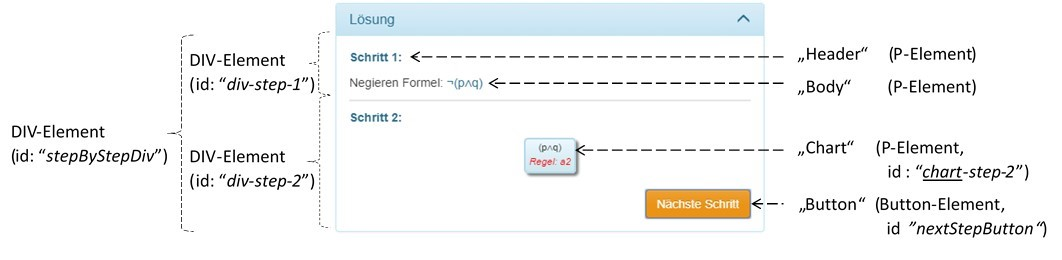
\includegraphics[width=1.0\textwidth]{StepByStepPanelAufbau}
\caption[Aufbau der StepByStepPanel]{Aufbau der ``Schritt für Schritt Lösung'' Panel}\label{fig:StepByStepPanelAufbau}
\end{figure}

Das Konzept für die ``Schritt für Schritt Lösung'' ist es, dass zuerst die vollständige Lösung mit allen Schritten erstellt und je nach Bestätigung der ``Nächste Schritt'' Button wird die Lösung teilweise eingeblendet.

\subsection{Controller}\label{subsec:Controller}

Controller (Klasse \textit{TableauController}) sind verantwortlich für die Steuerung der Anwendung durch den Benutzer und dieser wird für die Kommunikation zwischen den Model und View verwendet. Sie werten die Eingabedaten aus und leiten sie weiter. Änderungen der Modelldaten werden also vom Controller eingeleitet. View und Controller bilden zusammen die Benutzungsoberfläche. Das Klassendiagramm der \textit{TableauController} ist in Abbildung \ref{fig:KlassendiagrammControllerView} gezeigt.

\begin{lstlisting}[language=JavaScript, caption= TableauController Konstruktor, basicstyle=\scriptsize] 
function TableauController(TableauView) {
    this.view = TableauView;
    this.rootFormula = this.getRootOfParserTree(this.view.input.value);
    this.tableau = null;
    this.rootTableau = null;
    if (!InputError) {
        this.tableau = new TableauForPropositionalLogic(this.rootFormula);
        this.rootTableau = this.tableau.rootNode;
    }
    return this;
}
\end{lstlisting}

Im Konstruktor des Controllers wird zunächst seine Methode \textit{getRootOfParserTree()} aufgerufen. Diese Methode erhält die Eingabe, die im Attribut \textit{input} der \textit{TableauView} gekapselt wird, und führt die generierten Lexer und Parser aus um einen Parse-tree zu erhalten. Mit Hilfe von einer Instanz der Klasse  \textit{FormulaListener} besucht sie diesen Parse-tree, um eine Baumdarstellung der Eingabeformel zu erstellen. Dieser Baum wird im Attribut \textit{rootFormula} des Controller gespeichert. Danach wird eine Instanz der Klasse \textit{TableauForPropositionalLogic} initialisiert, um ein Tableau der Eingabeformel zu erstellen. Die Wurzel des Tableau wird im Attribut \textit{rootTableau} des Controller gespeichert.

\begin{lstlisting}[language=JavaScript, caption=getRootOfParserTree() (Klasse TableauController), basicstyle=\scriptsize] 
TableauController.prototype.getRootOfParserTree = function (inputString) {
    var errorListener = new ErrorListener();
    var chars = new antlr4.InputStream(inputString);
    var lexer = new FormulaGrammarLexer(chars);
    var tokens = new antlr4.CommonTokenStream(lexer);
    var parser = new FormulaGrammarParser(tokens);
    parser.buildParseTrees = true;
    var tree = parser.stat();
    var listener = new FormulaListener();
    antlr4.tree.ParseTreeWalker.DEFAULT.walk(listener, tree);
    var root = listener.stack.slice(-1).pop();
    return root;
};
\end{lstlisting}

Wenn der Anwender den Button ``Erfüllbarkeit'' betätigt, wird die Methode \textit{satisfiable()} des Controllers ausgeführt. Die Methode wird zuerst die Eingabeformel mittels Google Charts darstellen und die Panels der View einblenden und das Prüfergebnis, das man mittels Methode \textit{isSatisfiable()} der Klasse \textit{TableauForPropositionalLogic} erhält, in der GUI ausgeben. Anschließend wird sie die  Tableau-Darstellung einblenden. Abschließend, mit Hilfe der Methoden \textit{createSolutionStepHeaderP()}, \textit{createSolutionStepBodyP(}) der Klasse TableauView wird sie die ``Schritt für Schritt Lösung'' erstellen.

Wenn der Anwender den Button ``Tautologie'' betätigt, wird die Methode \textit{tautology()} des Controllers ausgeführt. Diese Methode analog zur Methode \textit{satisfiable()}, dann wird sie zuerst die Eingabeformel negieren und das Attribut \textit{rootFormula} mit der Negationsformel aktualisieren. Danach prüft sie die Erfüllbarkeit der negierten Formel und die Ergebnisse werden eingeblendet.
\begin{lstlisting}[language=JavaScript, caption=tautology() (Klasse TableauController), basicstyle=\scriptsize] 
TableauController.prototype.tautology = function () {
    // this.rootFormula = this.getRootOfParserTree(this.view.input.value);
    google.charts.setOnLoadCallback(drawFormulaChart);
    this.view.panelFormula.style.display = 'block';
    var formula = this.rootFormula.toFormulaString();
    this.rootFormula = this.rootFormula.getNegativeFormula();
    this.tableau = new TableauForPropositionalLogic(this.rootFormula);
    this.rootTableau = this.tableau.rootNode;
    this.view.panelResult.style.display = 'block';
    this.view.tautologyDiv.style.display = 'block';
    this.view.unsatisfiableDiv.style.display = 'none';
    this.view.satisfiableDiv.style.display = 'none';
    if (this.tableau.isSatisfiable()) {
        isTautology = TautologyOrSatisfiableEnum.FALSE;
        isSatifiable = TautologyOrSatisfiableEnum.NOTTESTED;
        this.view.tautologySpan.innerHTML = formula + " ist keine ";
    } else {
        isTautology = TautologyOrSatisfiableEnum.TRUE;
        isSatifiable = TautologyOrSatisfiableEnum.NOTTESTED;
        this.view.tautologySpan.innerHTML = formula + " ist eine ";
    }
    this.view.formula.innerHTML = "Negierte Formel: ";
    this.view.tableau.innerHTML = "Tableau der negierten Formel: ";
    this.view.panelTableau.style.display = 'block';
    google.charts.setOnLoadCallback(drawTableauChart);
    this.view.createSolutionStepHeaderP(this.view.stepByStepDiv);
    var text = "Negieren Formel:  <span  class='text-info'>" + this.rootFormula.toFormulaString() + "</span>";
    this.view.createSolutionStepBodyP(this.view.stepByStepDiv, text);
    chartNr = 2;
    stepNr++;
};
\end{lstlisting}

Weiterhin bietet die Klasse \textit{TableauController} noch die Methode \textit{toDisplayInput()}. Mit Hilfe des Lexers von ANTLR formatiert die Methode die Eingabeformel (z.B von p\&q nach p$\wedge$q). Diese formatierende Formel wird mittels der Klassen \textit{TableauView} eingeblendet.	